% Relatório - Análise estrutural do grafo p2p-Gnutella08 (layout acadêmico em duas colunas padrão WebMedia/ACM)
% Compilar com: pdflatex relatorio.tex (duas vezes). Figuras vêm de ../results.
\documentclass[10pt,a4paper,twocolumn]{article}
\usepackage[utf8]{inputenc}
\usepackage[T1]{fontenc}
\usepackage{mathptmx}
\usepackage[scaled=0.92]{helvet}
\usepackage{courier}
\usepackage{graphicx,booktabs,xcolor,hyperref,amsmath,float,geometry,titlesec,fancyhdr,caption,microtype}
\geometry{top=2.0cm,bottom=2.0cm,left=1.7cm,right=1.7cm,columnsep=0.65cm}
\graphicspath{{../results/}}

\renewcommand{\figurename}{Figura}
\renewcommand{\tablename}{Tabela}
\renewcommand{\refname}{REFERÊNCIAS}

\titleformat{\section}{\normalfont\normalsize\bfseries\uppercase}{\thesection}{0.6em}{}
\titleformat{\subsection}{\normalfont\small\bfseries}{\thesubsection}{0.5em}{}
\titlespacing*{\section}{0pt}{1.1em}{0.4em}
\titlespacing*{\subsection}{0pt}{0.8em}{0.3em}

\captionsetup{font=footnotesize,labelfont=bf}
\hypersetup{colorlinks=true,linkcolor=black,citecolor=black,urlcolor=blue!60!black}

\pagestyle{fancy}
\fancyhf{}
\fancyhead[L]{\footnotesize\itshape Análise Estrutural da Rede Gnutella (p2p-Gnutella08)}
\fancyhead[R]{\footnotesize\itshape Valque Pinho dos Santos Junior}
\fancyfoot[C]{\footnotesize\thepage}
\renewcommand{\headrulewidth}{0.4pt}

\begin{document}

\twocolumn[
\begin{@twocolumnfalse}
\begin{center}
{\LARGE\bfseries Análise Estrutural da Rede Gnutella (p2p-Gnutella08)\par}
\vspace{0.55em}
{\large\bfseries Valque Pinho dos Santos Junior\par}
\vspace{0.2em}
{\small Matrícula: 222217667\par}
{\small Repositório Git: \url{https://github.com/valquepinho/trabalhomata53}\par}
\end{center}
\vspace{0.6em}
\end{@twocolumnfalse}
]
\thispagestyle{plain}

\section*{RESUMO}
Este relatório apresenta uma análise estrutural e algorítmica do grafo \texttt{p2p-Gnutella08} (SNAP/Stanford), composto por 6.301 vértices e 20.777 arestas. Avaliam-se métricas topológicas nas versões dirigida e não-dirigida, o desempenho empírico de nove algoritmos clássicos de grafos frente às suas complexidades teóricas, bem como propriedades de \emph{small-world}, distribuição de graus em cauda pesada, robustez sob falhas aleatórias e ataques direcionados (incluindo número de componentes, fração de nós isolados e \emph{boxplots} com média $\pm$ desvio padrão) e comparação com modelos clássicos.

\medskip\noindent\textbf{PALAVRAS-CHAVE:} Teoria dos Grafos, p2p-Gnutella08, Redes Complexas, Small-World, Lei de Potência, Robustez.

\section{Determinação do grafo}
A partir do número de matrícula $M = 222217667$, aplica-se a regra de mapeamento estabelecida na disciplina:
\begin{align*}
f(M) = \big(&(\text{soma dos dígitos de } M) \\
            &\times (\text{últimos 2 dígitos de } M + 1)\big) \bmod 129
\end{align*}
(adotando-se 129 caso o resto seja 0). Substituindo $M = 222217667$:
\begin{align*}
f(222217667) &= \big((2+2+2+2+1+7+6+6+7) \\
             &\quad \times (67 + 1)\big) \bmod 129 \\
             &= (35 \times 68) \bmod 129 \\
             &= 2380 \bmod 129 = 58.
\end{align*}
O índice \textbf{58} corresponde exatamente ao dataset \texttt{p2p-Gnutella08} do SNAP (\emph{Internet peer-to-peer networks}, dirigido, 6.301 vértices e 20.777 arestas, disponível em \url{https://snap.stanford.edu/data/p2p-Gnutella08.html}).

\medskip\noindent\textbf{Repositório (código, dados tratados e README):} \url{https://github.com/valquepinho/trabalhomata53}.

\section{Descrição do grafo original e tratamento realizado}
O grafo é o \emph{p2p-Gnutella08} (SNAP/Stanford): um instantâneo de 8 de agosto de 2002 da rede de compartilhamento de arquivos Gnutella, em que cada vértice é um hospedeiro (\emph{peer}) e cada aresta é uma conexão entre dois hospedeiros \cite{leskovec2007,ripeanu2002}. O arquivo é uma lista de arestas dirigidas com 6.301 vértices e 20.777 arestas.

\paragraph{Tratamento.} O arquivo foi lido com um \emph{script} próprio (\texttt{src/grafo.py}) que ignora comentários, remove laços e arestas duplicadas e reindexa os vértices em $0,\dots,n-1$. O resultado foi: 20.777 linhas de aresta lidas, \textbf{0 laços, 0 duplicatas e 0 pares recíprocos} (nunca ocorrem $u\to v$ e $v\to u$ juntos). Portanto o grafo tratado coincide com o original: $n=6.301$, $m=20.777$ arestas dirigidas e 20.777 arestas na versão não-dirigida. Os valores conferem com a página oficial do SNAP (6.301 vértices, 20.777 arestas, 2.383 triângulos, clustering médio 0,0109).

\paragraph{Cuidado com a orientação.} O cabeçalho do arquivo diz que \emph{cada par não ordenado de vértices é salvo uma vez}. Isso explica a ausência de pares recíprocos e indica que a orientação das arestas deve ser interpretada com cautela. Por isso as medidas foram calculadas nas duas versões (dirigida e não-dirigida), e cada resultado diz qual foi usada.

\paragraph{Obtenção do arquivo.} O arquivo \texttt{p2p-Gnutella08.txt.gz} utilizado foi obtido por meio de download direto no site oficial do SNAP (\url{https://snap.stanford.edu/data/p2p-Gnutella08.html}). A integridade do arquivo foi confirmada pelas contagens oficiais (6.301 vértices, 20.777 arestas, 2.383 triângulos e clustering médio 0,0109), e o hash SHA-256 está registrado no README.

\section{Metodologia}
\begin{itemize}
\item \textbf{Implementação.} BFS, DFS, verificação de eulerianidade, Dijkstra, Bellman-Ford, Floyd-Warshall, Tarjan, Kruskal e Prim foram implementados \emph{à mão} em Python, sem recursão (\texttt{src/algoritmos.py}). O \texttt{networkx} foi usado apenas nos testes automáticos (13 testes comparando com a biblioteca em grafos aleatórios, todos passando) e para calcular o \emph{layout} da visualização.
\item \textbf{Versão do grafo.} Graus, componentes fortes (Tarjan) e BFS/DFS usam o grafo dirigido; clustering, triângulos, MST, \emph{small-world} e robustez usam a versão não-dirigida.
\item \textbf{Distâncias.} O grafo dirigido não é fortemente conexo, então muitos pares têm distância infinita. Diâmetro, raio e comprimento médio foram calculados por BFS a partir de \emph{todos} os vértices em três contextos: (a) dirigido, pares alcançáveis; (b) não-dirigido, maior componente fracamente conexa (WCC); (c) dirigido, maior componente fortemente conexa (SCC). O raio não é definido em (a).
\item \textbf{Pesos.} O grafo não tem pesos: Dijkstra, Bellman-Ford e Floyd-Warshall usam peso 1. Kruskal e Prim usam pesos inteiros aleatórios entre 1 e 10 (semente fixa), senão a árvore seria trivial; como há 2 componentes, o resultado é uma floresta geradora mínima, e os dois algoritmos são verificados no código (mesmo peso total).
\item \textbf{Tempo real.} Cada algoritmo foi medido 30 vezes (\texttt{perf\_counter}, após uma execução de aquecimento) em subgrafos de 500 a 6.301 vértices (os $k$ primeiros vértices de uma BFS a partir do vértice de maior grau). Com $n\ge30$ o IC de 95\% usa a Normal, $\bar x\pm z_{\alpha/2}\,s/\sqrt n$ com $z=1{,}96$; com $n<30$ e $\sigma$ desconhecido usa a $t$-Student com $n-1$ graus de liberdade. O desvio padrão $s$ é o amostral. O Floyd-Warshall, por custar $O(n^3)$, foi medido com 10 repetições (até $n=400$) e 5 (acima), portanto com a $t$-Student.
\item \textbf{\emph{Small-world}.} Implementado sem bibliotecas de grafos: $C$ (clustering médio) e $L$ (comprimento médio) da maior componente, comparados a (i) $G(n,m)$ de Erdős--Rényi, (ii) um modelo nulo que preserva a sequência de graus (troca de arestas) e (iii) as aproximações $C_{rand}\approx\langle k\rangle/n$ e $L_{rand}\approx\ln n/\ln\langle k\rangle$. O índice é $\sigma=(C/C_{rand})/(L/L_{rand})$. Os modelos nulos usam 5 réplicas, com $L$ estimado por 300 fontes de BFS por réplica.
\item \textbf{Lei de potência.} Estimador de máxima verossimilhança discreto, com $x_{min}$ escolhido pela menor distância de Kolmogorov--Smirnov (KS), como em Clauset, Shalizi e Newman. A cauda é comparada a exponencial e log-normal pela razão de verossimilhança normalizada de Vuong.
\item \textbf{Robustez.} Remoção de 5\% dos vértices ($r = \lfloor 0{,}05 \times n \rceil = 315$): (a) aleatória, com $T = 30$ repetições; (b) os 5\% de maior grau; (c) os 5\% de maior intermediação (Brandes com 500 fontes amostradas). Os ataques são estáticos (o \emph{ranking} é calculado uma vez no grafo original). Conforme o Apêndice~C, medem-se: \emph{Métrica~A} (tamanho da maior componente fraca e forte), \emph{Métrica~B} (número de componentes conexas), \emph{Métrica~C} (distância média $L$ na maior WCC e eficiência global) e \emph{Métrica~D} (fração de nós isolados entre os vértices restantes), reportadas em tabela e em \emph{boxplots} com média $\pm$ desvio padrão.
\end{itemize}

\section{Resultados}
\subsection{Parte I -- Análise estrutural obrigatória}
A Tabela~\ref{tab:medidas} reúne todas as medidas pedidas e indica que todas foram computadas.

\begin{table*}[t]\centering\scriptsize
\caption{Medidas da Parte I e indicação de que foram computadas.}\label{tab:medidas}
\begin{tabular}{p{3.4cm}cp{5.2cm}p{5.0cm}}\toprule
\textbf{Medida} & \textbf{Comp.?} & \textbf{Valor} & \textbf{Observação} \\\midrule
Número de vértices & Sim & 6.301 & Após remoção de laços/duplicatas \\
Número de arestas & Sim & 20.777 dirigidas; 20.777 não-dirigidas & 0 pares recíprocos ($u\to v$ e $v\to u$) \\
Grau mín./máx./médio (entrada) & Sim & mín 0 / máx 91 / média 3,297 & Grau de entrada \\
Grau mín./máx./médio (saída) & Sim & mín 0 / máx 48 / média 3,297 & Grau de saída \\
Grau mín./máx./médio (não-dir.) & Sim & mín 1 / máx 97 / média 6,595 & Vizinhos distintos \\
Distribuição de graus & Sim & ver Figura~\ref{fig:graus} e \texttt{graus.csv} & Histograma e CCDF log-log \\
Densidade & Sim & dir.\ 0,0005234; não-dir.\ 0,001047 & $m/(n(n-1))$ e $2m/(n(n-1))$ \\
Nº de componentes conexas & Sim & 2 fracas; 4.234 fortes & Fracas: BFS não-dirigida; fortes: Tarjan \\
Tamanho de cada componente & Sim & fracas: [6299, 2]; fortes: maior 2068, 4.233 unit. & Lista completa em \texttt{componentes.csv} \\
Diâmetro & Sim & dir.\ (alcançáveis) 20; não-dir.\ (WCC) 9; SCC 19 & Dirigido não é fortemente conexo \\
Raio & Sim & não-dir.\ (maior WCC) 6; maior SCC 12 & Indefinido no dirigido completo \\
Comprimento médio dos caminhos & Sim & dir.\ 6,6322; não-dir.\ 4,6430; SCC 6,4339 & Média sobre pares alcançáveis ($s\neq t$) \\
Diâmetro efetivo (percentil 90) & Sim & dirigido 8,493; não-dirigido 5,486 & Medida extra, comparável ao SNAP \\
Coef.\ de clustering médio & Sim & 0,01087 (todos); 0,01503 ($\text{grau}\ge 2$); trans.\ 0,02066 & Versão não-dirigida; grau $<2$ tem $C=0$ \\
Número de triângulos & Sim & 2.383 & Viável (grafo esparso); não-dirigido \\
Visualização do grafo & Sim & \texttt{visualizacao.png} & Subgrafo de 300 vértices (BFS do hub) \\
Eulerianidade & Sim & circuito (dir.): não; 6.133 vértices desbalanceados & Parte II \\\bottomrule
\end{tabular}
\end{table*}

\paragraph{Respostas às perguntas obrigatórias da Parte I.}
\begin{itemize}
\item \textbf{Vértices e arestas:} 6.301 vértices; 20.777 arestas (dirigidas e não-dirigidas).
\item \textbf{Graus:} entrada de 0 a 91 (média 3,297); saída de 0 a 48 (média 3,297); não-dirigido de 1 a 97 (média 6,595; mediana 3). As médias de entrada e saída são iguais porque cada aresta soma um em cada lado.
\item \textbf{Densidade:} $5{,}23\times10^{-4}$ (dirigida) e $1{,}05\times10^{-3}$ (não-dirigida): o grafo é muito esparso.
\item \textbf{Componentes:} 2 componentes fracamente conexas (6.299 e 2 vértices) e 4.234 fortemente conexas (uma com 2.068 vértices, 32,8\% do total, e 4.233 unitárias).
\item \textbf{Diâmetro / raio / $L$:} dirigido (pares alcançáveis) diâmetro 20 e $L=6{,}63$; não-dirigido na maior WCC diâmetro 9, raio 6 e $L=4{,}64$; maior SCC diâmetro 19, raio 12 e $L=6{,}43$. O diâmetro efetivo (percentil 90) é 5,49 no não-dirigido.
\item \textbf{Clustering e triângulos:} clustering médio 0,01087 (0,01503 considerando só vértices de grau $\ge2$), transitividade 0,02066 e 2.383 triângulos.
\end{itemize}

\begin{figure*}[t]\centering
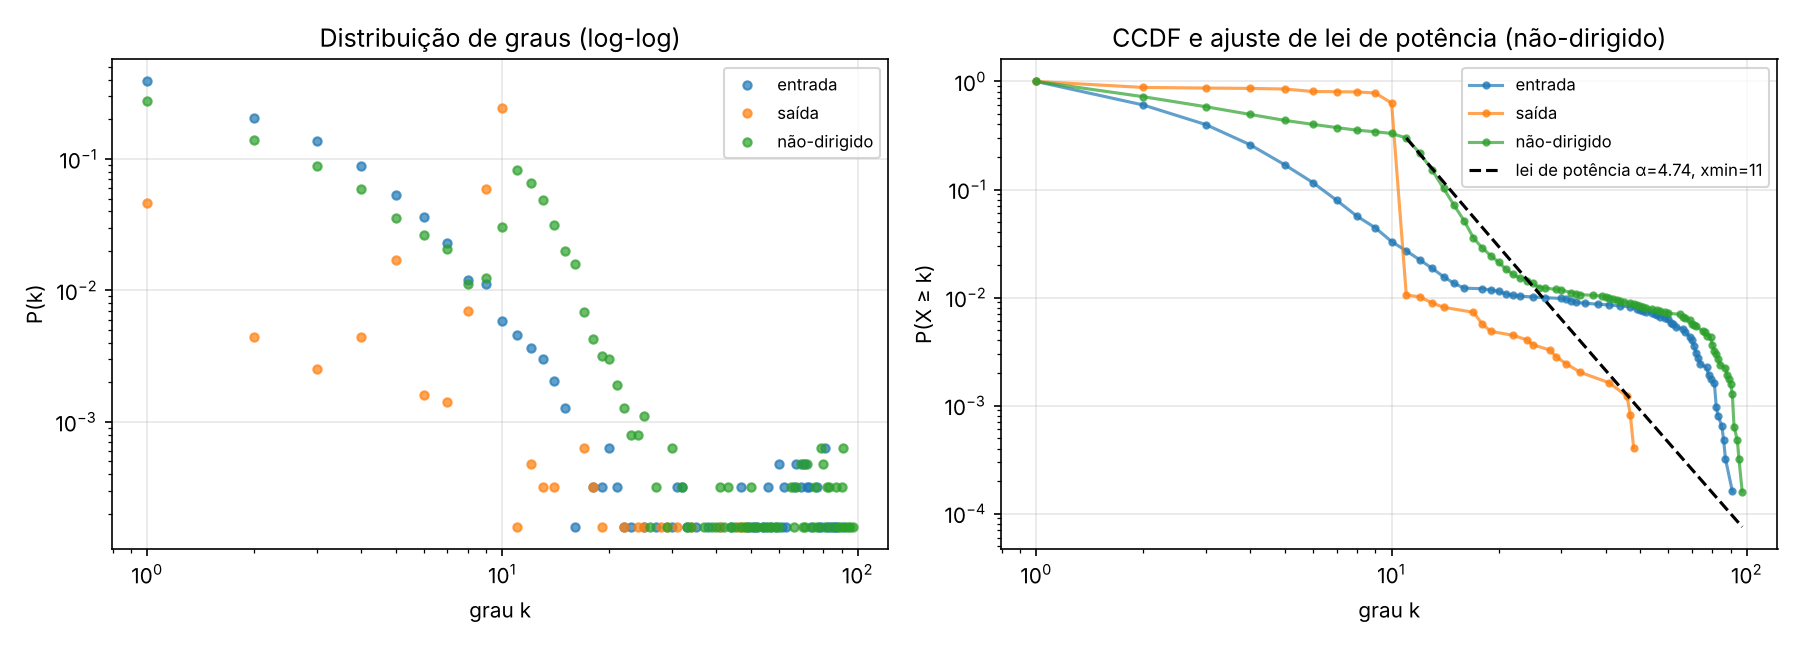
\includegraphics[width=0.92\textwidth]{distribuicao_graus.png}
\caption{Distribuição de graus (esquerda, log-log) e CCDF com o ajuste de lei de potência para o grau não-dirigido (direita).}\label{fig:graus}
\end{figure*}
\noindent\textbf{Comentário da Figura~\ref{fig:graus}.} O grau de entrada decai de forma gradual e tem cauda longa (máximo 91). O grau de saída é muito diferente: 3.836 vértices (60,9\%) têm saída 0 e, entre os 2.465 restantes, 62\% têm saída \emph{exatamente} 10 e 98,9\% têm saída $\le10$ (só 26 passam de 10). Isso aparece como o ponto isolado em $k=10$ no gráfico da esquerda e como a queda abrupta da CCDF de saída em $k\approx10$. A CCDF não-dirigida tem um patamar entre $k\approx25$ e $k\approx70$, ou seja, um pequeno grupo de ``super-hubs'' (cerca de 1\% dos vértices, ${\sim}60$) com graus entre ${\sim}25$ e 97; os dez maiores graus ficam todos entre 90 e 97.

\begin{figure*}[t]\centering
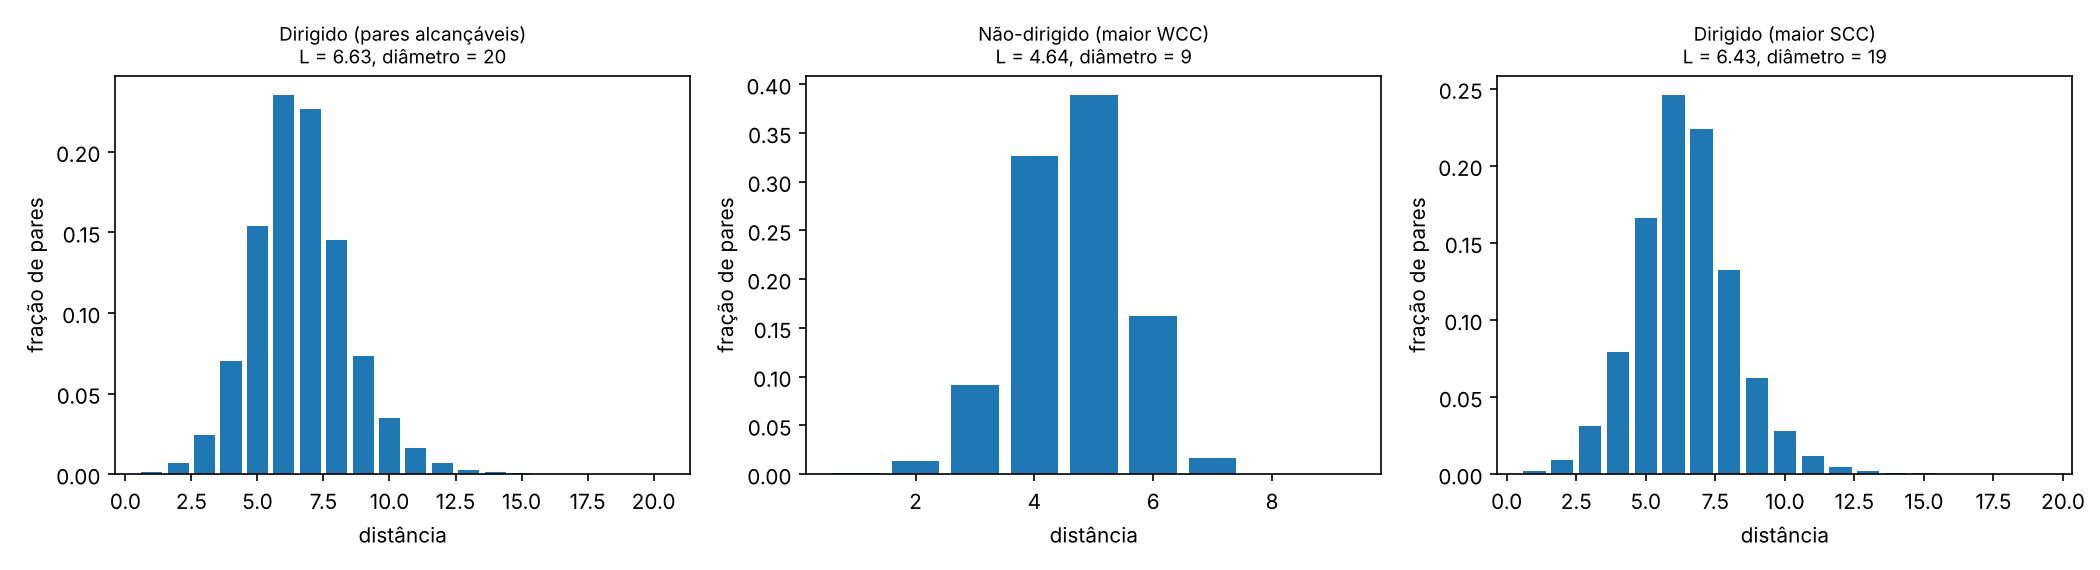
\includegraphics[width=0.95\textwidth]{distancias.png}
\caption{Distribuição das distâncias nos três contextos.}\label{fig:dist}
\end{figure*}
\noindent\textbf{Comentário da Figura~\ref{fig:dist}.} No grafo não-dirigido, 82,1\% dos pares alcançáveis estão a no máximo 5 saltos, 98,3\% a no máximo 6 e 99,95\% a no máximo 7; a moda é 5. As distâncias dirigidas são maiores (média 6,63, diâmetro 20) porque o caminho precisa respeitar o sentido das arestas.

\begin{figure}[H]\centering
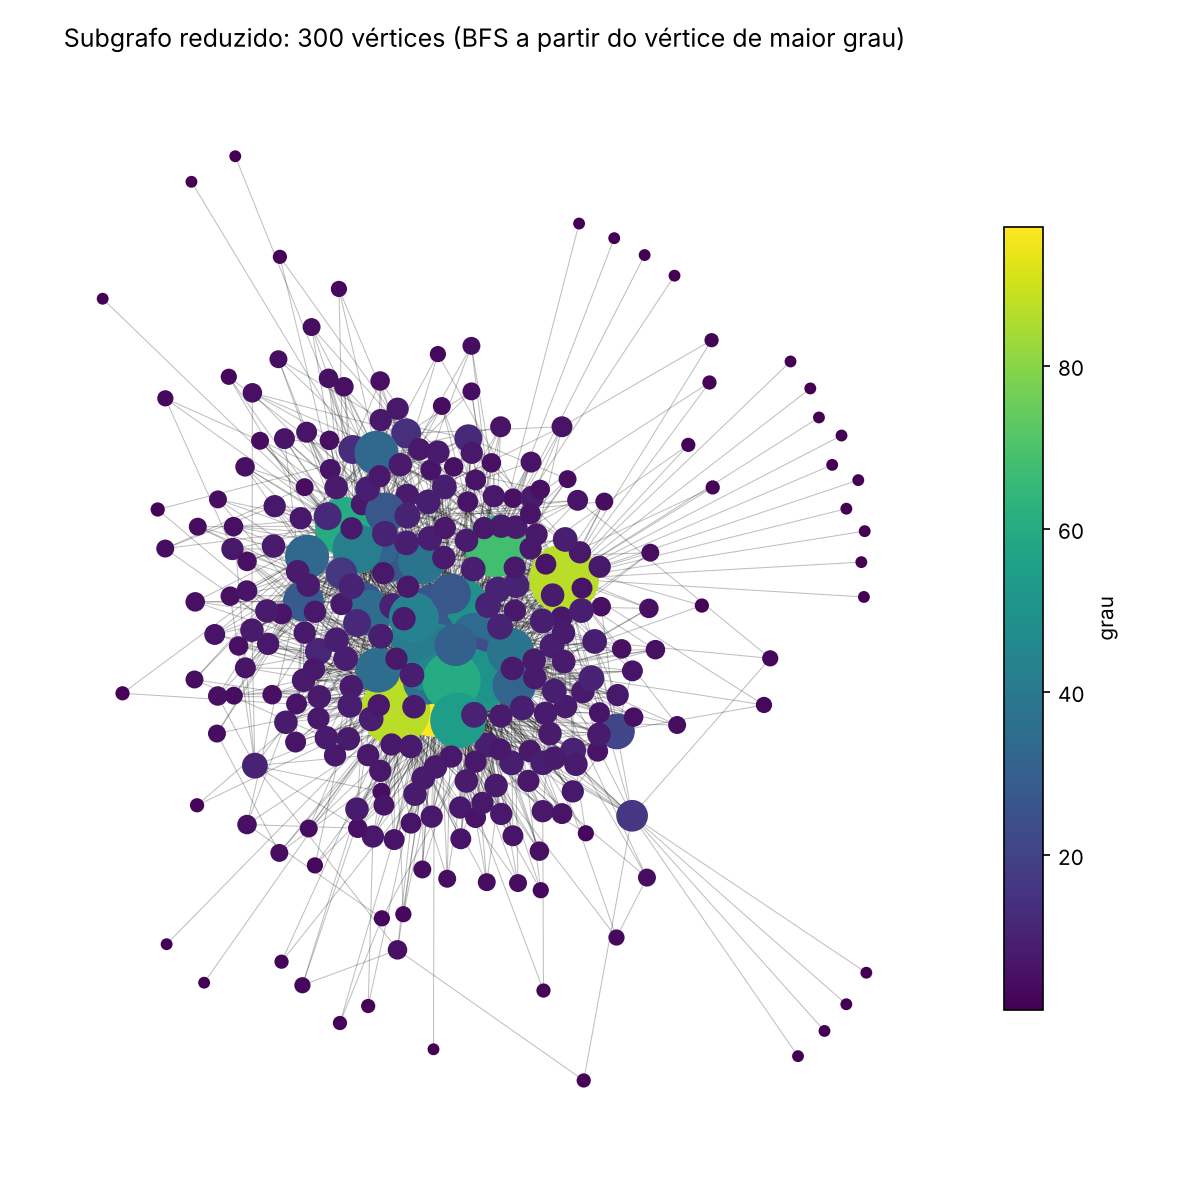
\includegraphics[width=.62\linewidth]{visualizacao.png}
\caption{Versão reduzida do grafo: 300 vértices obtidos por BFS a partir do vértice de maior grau; cor e tamanho indicam o grau.}\label{fig:vis}
\end{figure}
\noindent\textbf{Comentário da Figura~\ref{fig:vis}.} Há um núcleo denso em torno dos hubs e muitos vértices periféricos de grau 1 ou 2 pendurados nele. O grafo completo é uma ``bola de pelos'' ilegível, por isso a amostra.

\subsection{Parte II -- Algoritmos da disciplina}
A Tabela~\ref{tab:tempos} mostra o tempo médio no maior tamanho medido, com desvio padrão e IC de 95\%. A Figura~\ref{fig:bench} compara o tempo observado com a curva teórica ajustada ($T=c\cdot f(n,m)$, com $c$ por mínimos quadrados).

\begin{table*}[t]\centering\footnotesize
\caption{Tempo real por algoritmo no maior tamanho medido (Floyd-Warshall: $n=1400$).}\label{tab:tempos}
\begin{tabular}{llrrrrllr}\toprule
\textbf{Algoritmo} & \textbf{Teórica} & \textbf{$n$} & \textbf{Rep.} & \textbf{Média (ms)} & \textbf{Desvio (ms)} & \textbf{IC 95\% (ms)} & \textbf{Distribuição} & \textbf{Exp.\ emp.} \\\midrule
BFS & $O(n+m)$ & 6301 & 30 & 0,359 & 0,573 & [0,154; 0,564] & Normal ($z$) & 1,22 \\
DFS & $O(n+m)$ & 6301 & 30 & 1,186 & 1,823 & [0,533; 1,838] & Normal ($z$) & 1,24 \\
Eulerianidade & $O(n+m)$ & 6301 & 30 & 3,618 & 0,143 & [3,566; 3,669] & Normal ($z$) & 0,99 \\
Tarjan & $O(n+m)$ & 6301 & 30 & 5,695 & 0,710 & [5,440; 5,949] & Normal ($z$) & 0,97 \\
Dijkstra & $O((n+m)\log n)$ & 6301 & 30 & 1,170 & 1,820 & [0,519; 1,822] & Normal ($z$) & 1,37 \\
Bellman-Ford & $O(n\cdot m)$ & 6301 & 30 & 3,897 & 3,698 & [2,574; 5,221] & Normal ($z$) & 0,81 \\
Kruskal & $O(m\log m)$ & 6301 & 30 & 8,553 & 0,349 & [8,428; 8,678] & Normal ($z$) & 0,88 \\
Prim & $O(m\log n)$ & 6301 & 30 & 22,659 & 3,538 & [21,393; 23,925] & Normal ($z$) & 1,04 \\
Floyd-Warshall & $O(n^3)$ & 1400 & 5 & 2771,360 & 152,607 & [2581,874; 2960,846] & $t$-Student ($\text{gl}=4$) & 3,10 \\\bottomrule
\end{tabular}
\end{table*}

\begin{figure*}[t]\centering
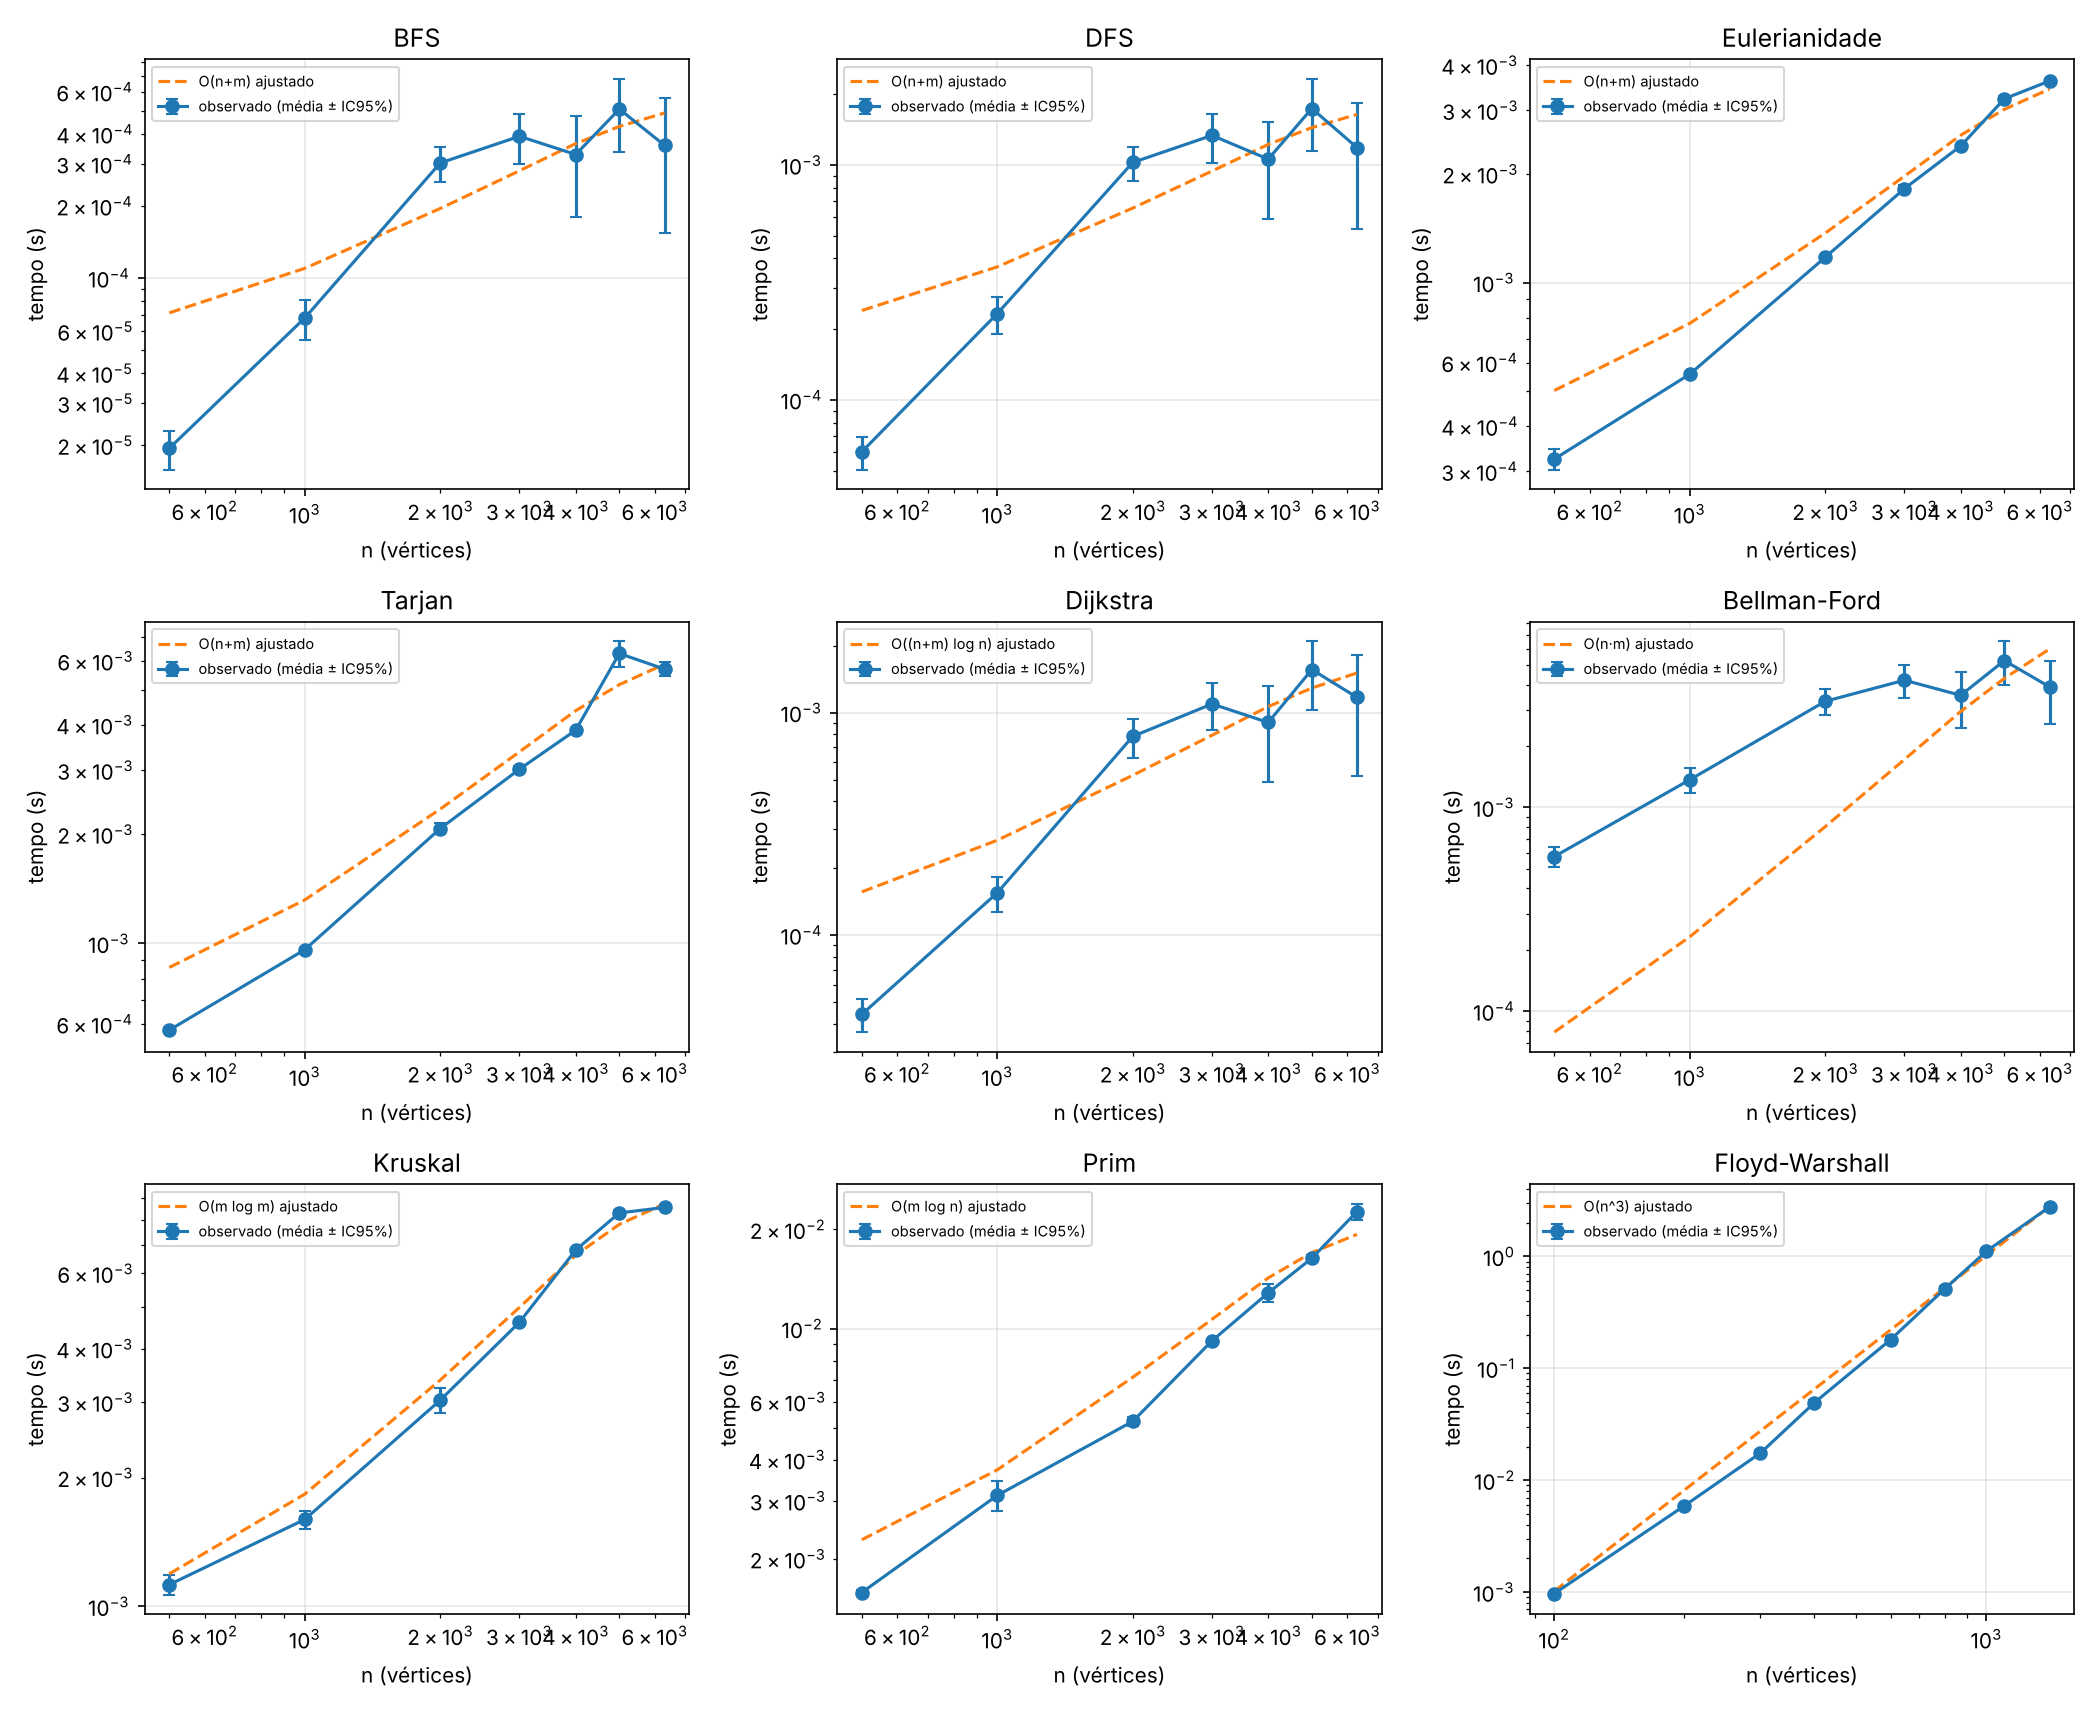
\includegraphics[width=0.92\textwidth]{benchmark.png}
\caption{Tempo observado (média $\pm$ IC 95\%) e complexidade teórica ajustada, em escala log-log.}\label{fig:bench}
\end{figure*}

\noindent\textbf{Complexidade teórica $\times$ observada.}
\begin{itemize}
\item \textbf{Tarjan, eulerianidade, Kruskal e Prim} (lineares ou quase) seguem bem o modelo: $R^2$ de 0,93 a 0,99 e expoente empírico próximo de 1.
\item \textbf{BFS, DFS e Dijkstra} têm $R^2$ mais baixo (0,72; 0,69; 0,78) e desvios padrão maiores que a média. A causa é o grafo, não o algoritmo: 60,9\% dos vértices têm grau de saída 0, então uma fonte sorteada alcança poucos vértices ou muitos, e o trabalho real depende de quem foi sorteado. O ajuste continua compatível com crescimento linear, mas o IC é largo (por exemplo, BFS em $n=6.301$: média 0,36 ms, IC [0,15; 0,56] ms).
\item \textbf{Dijkstra} com peso 1 equivale a BFS, só que com um \emph{heap}, e é mais lento que a BFS (1,17 ms contra 0,36 ms em $n=6.301$), por causa do custo do \emph{heap}.
\item \textbf{Bellman-Ford:} o modelo de pior caso $O(n\cdot m)$ ajusta mal ($R^2<0$) porque a implementação para quando uma rodada não altera nada. Ela precisou de apenas 2,9 a 6,4 rodadas em média, contra $n-1$ no pior caso. Com o custo real, $m\cdot\text{rodadas}$, o $R^2$ sobe para 0,98. O pior caso teórico não se manifesta neste grafo (diâmetro pequeno).
\item \textbf{Floyd-Warshall:} expoente empírico 3,10 ($R^2=0{,}998$), confirmando $O(n^3)$. Na forma como foi implementado, o laço em $k$ é explícito e as atualizações $(i,j)$ são vetorizadas com \texttt{numpy}. No grafo inteiro ($n=6.301$), uma \emph{única} execução levou \textbf{402 s} (${\approx}6{,}7$ min), sem IC por ser uma só medição. A extrapolação cúbica a partir de $n=1.400$ (2,77 s) daria ${\approx}253$ s; o tempo medido foi maior, possivelmente porque a matriz ($6.301^2$ valores de 4 bytes, 159 MB) deixa de caber na memória \emph{cache}, o que é uma hipótese, não foi investigado.
\end{itemize}
\noindent\textbf{Eulerianidade.} O grafo \emph{não} tem circuito nem caminho euleriano, nem como dirigido (6.133 vértices com grau de entrada diferente do de saída; 4.238 com diferença maior que 1) nem como não-dirigido (3.824 vértices de grau ímpar; seriam permitidos no máximo 2).

\noindent\textbf{Observação sobre o IC.} Com exatamente 30 repetições, o critério $n\ge30$ do enunciado manda usar a Normal; com $n=5$ ou $10$ (Floyd-Warshall) usa-se a $t$ ($t_{0{,}025;4}=2{,}776$, $t_{0{,}025;9}=2{,}262$), cujos ICs são mais largos.

\subsection{Parte III -- Análise estrutural}

\paragraph{1. Há indícios de \emph{small-world}?}
\begin{table}[t]\centering\scriptsize
\caption{Comparação com modelos nulos para o \emph{small-world}.}\label{tab:sw}
\begin{tabular}{lrrr}\toprule
Modelo & $C$ & $L$ & $\sigma$ \\\midrule
Grafo real (maior WCC, não-dir.) & 0,01087 & 4,643 & -- \\
Erdős--Rényi $G(n,m)$ (5 réplicas) & 0,00116 & 4,848 & 9,80 \\
Preserva graus (5 réplicas) & 0,00465 & 4,308 & 2,17 \\
Analítico ($\langle k\rangle/n$; $\ln n/\ln\langle k\rangle$) & 0,00105 & 4,637 & 10,37 \\\bottomrule
\end{tabular}
\end{table}
\noindent\textbf{Sim, com ressalvas.} O comprimento médio ($4{,}64$) é praticamente o de um grafo aleatório com o mesmo tamanho (4,85), e o clustering é cerca de 9 vezes maior que o aleatório, o que dá $\sigma\approx9{,}8>1$. Mas há duas ressalvas. (i) O valor absoluto de $C$ é minúsculo (0,011), muito longe dos ${\sim}0{,}45$ de uma rede Watts--Strogatz típica; o ganho relativo vem de o aleatório ser quase zero. (ii) Contra o modelo que preserva a sequência de graus, $\sigma$ cai para 2,17 e $L$ real é \emph{maior} que o do nulo (4,64 contra 4,31): boa parte do ``mundo pequeno'' é efeito dos hubs. Concluo que há indício, mas fraco, de \emph{small-world} no sentido de Watts--Strogatz; o que é claro é o diâmetro pequeno.

\noindent\textbf{Implicação prática.} 99,95\% dos pares alcançáveis estão a até 7 saltos. Numa rede P2P, isso significa que uma busca por inundação com poucos saltos de validade (TTL) alcança praticamente toda a rede, o que é bom para localizar arquivos, mas custoso em tráfego, e que informações (ou \emph{malware}) se propagam rapidamente.

\paragraph{2. A distribuição de graus sugere uma lei de potência?}
\begin{table*}[t]\centering\footnotesize
\caption{Ajuste de lei de potência discreta à cauda ($R>0$ favorece a lei de potência). \textsuperscript{*}$\alpha$ no limite superior do otimizador.}\label{tab:pl}
\begin{tabular}{lrrrrr}\toprule
Grau & $x_{\min}$ & $\alpha$ & KS & $R$ vs.\ exponencial & $R$ vs.\ log-normal \\\midrule
Não-dirigido & 11 & 4,74 & 0,067 & $+442$ ($z=10{,}8$) & $+12{,}7$ ($z=8{,}0$) \\
Entrada & 4 & 2,84 & 0,034 & $+525$ ($z=10{,}4$) & $+5{,}5$ ($z=3{,}5$) \\
Saída & 10 & 12,0\textsuperscript{*} & 0,319 & $+26$ ($z=0{,}3$) & $-228$ ($z=-4{,}4$) \\\bottomrule
\end{tabular}
\end{table*}
\noindent\textbf{Resposta: parcialmente, e não de forma conclusiva.} O grau de \emph{entrada} é o mais compatível: $\alpha\approx2{,}84$ com KS baixo (0,034) e cauda de 1.614 vértices. O grau não-dirigido ajusta $\alpha\approx4{,}74$ a partir de $k=11$, com KS maior (0,067), e a Figura~\ref{fig:graus} mostra o patamar de super-hubs que uma lei de potência pura não explica. O grau de \emph{saída} claramente não é lei de potência (KS 0,32; $\alpha$ foi para o limite do otimizador), por causa do limite de cerca de 10 conexões de saída. A lei de potência vence a exponencial com folga, mas contra a log-normal a vantagem é pequena e o parâmetro $\mu$ da log-normal foi parar no limite da busca ($-12$): truncada numa cauda, a log-normal tende a imitar uma lei de potência, então essa comparação é \emph{inconclusiva}. Não foi feito o teste de aderência por \emph{bootstrap} de Clauset et al., portanto não afirmo que a lei de potência seja plausível, só que a cauda é pesada.

\paragraph{3. O grafo é robusto?}
\begin{table*}[t]\centering\scriptsize
\setlength{\tabcolsep}{4.5pt}
\caption{Impacto da remoção de 5\% dos vértices ($r=315$) nas métricas do Apêndice~C: maior componente (Métrica~A: WCC/$n$, WCC/restantes e SCC/$n$), número de componentes (Métrica~B), distâncias (Métrica~C: $L$ na maior WCC e eficiência global) e fração de nós isolados entre os restantes (Métrica~D). Na remoção aleatória reporta-se média $\pm$ desvio padrão das 30 repetições.}\label{tab:rob}
\begin{tabular}{lccccccc}\toprule
Cenário (5\% = 315 vértices) & WCC/$n$ & WCC/rest. & Nº comp. & SCC/$n$ & $L$ (WCC) & Efic.\ glob. & Isolados \\\midrule
Sem remoção & 0,9997 & 0,9997 & 2 & 0,328 & 4,66 & 0,226 & 0,0000 \\
Aleatória (30 rep., média $\pm$ DP) & 0,936 $\pm$ 0,002 & 0,985 $\pm$ 0,002 & 89,93 $\pm$ 14,07 & 0,301 $\pm$ 0,002 & 4,68 $\pm$ 0,03 & 0,222 $\pm$ 0,002 & 0,0145 $\pm$ 0,0023 \\
Maior grau & 0,893 & 0,940 & 357 & 0,163 & 5,39 & 0,183 & 0,0585 \\
Maior intermediação & 0,868 & 0,913 & 510 & 0,193 & 5,12 & 0,187 & 0,0834 \\\bottomrule
\end{tabular}
\end{table*}
\begin{figure*}[t]\centering
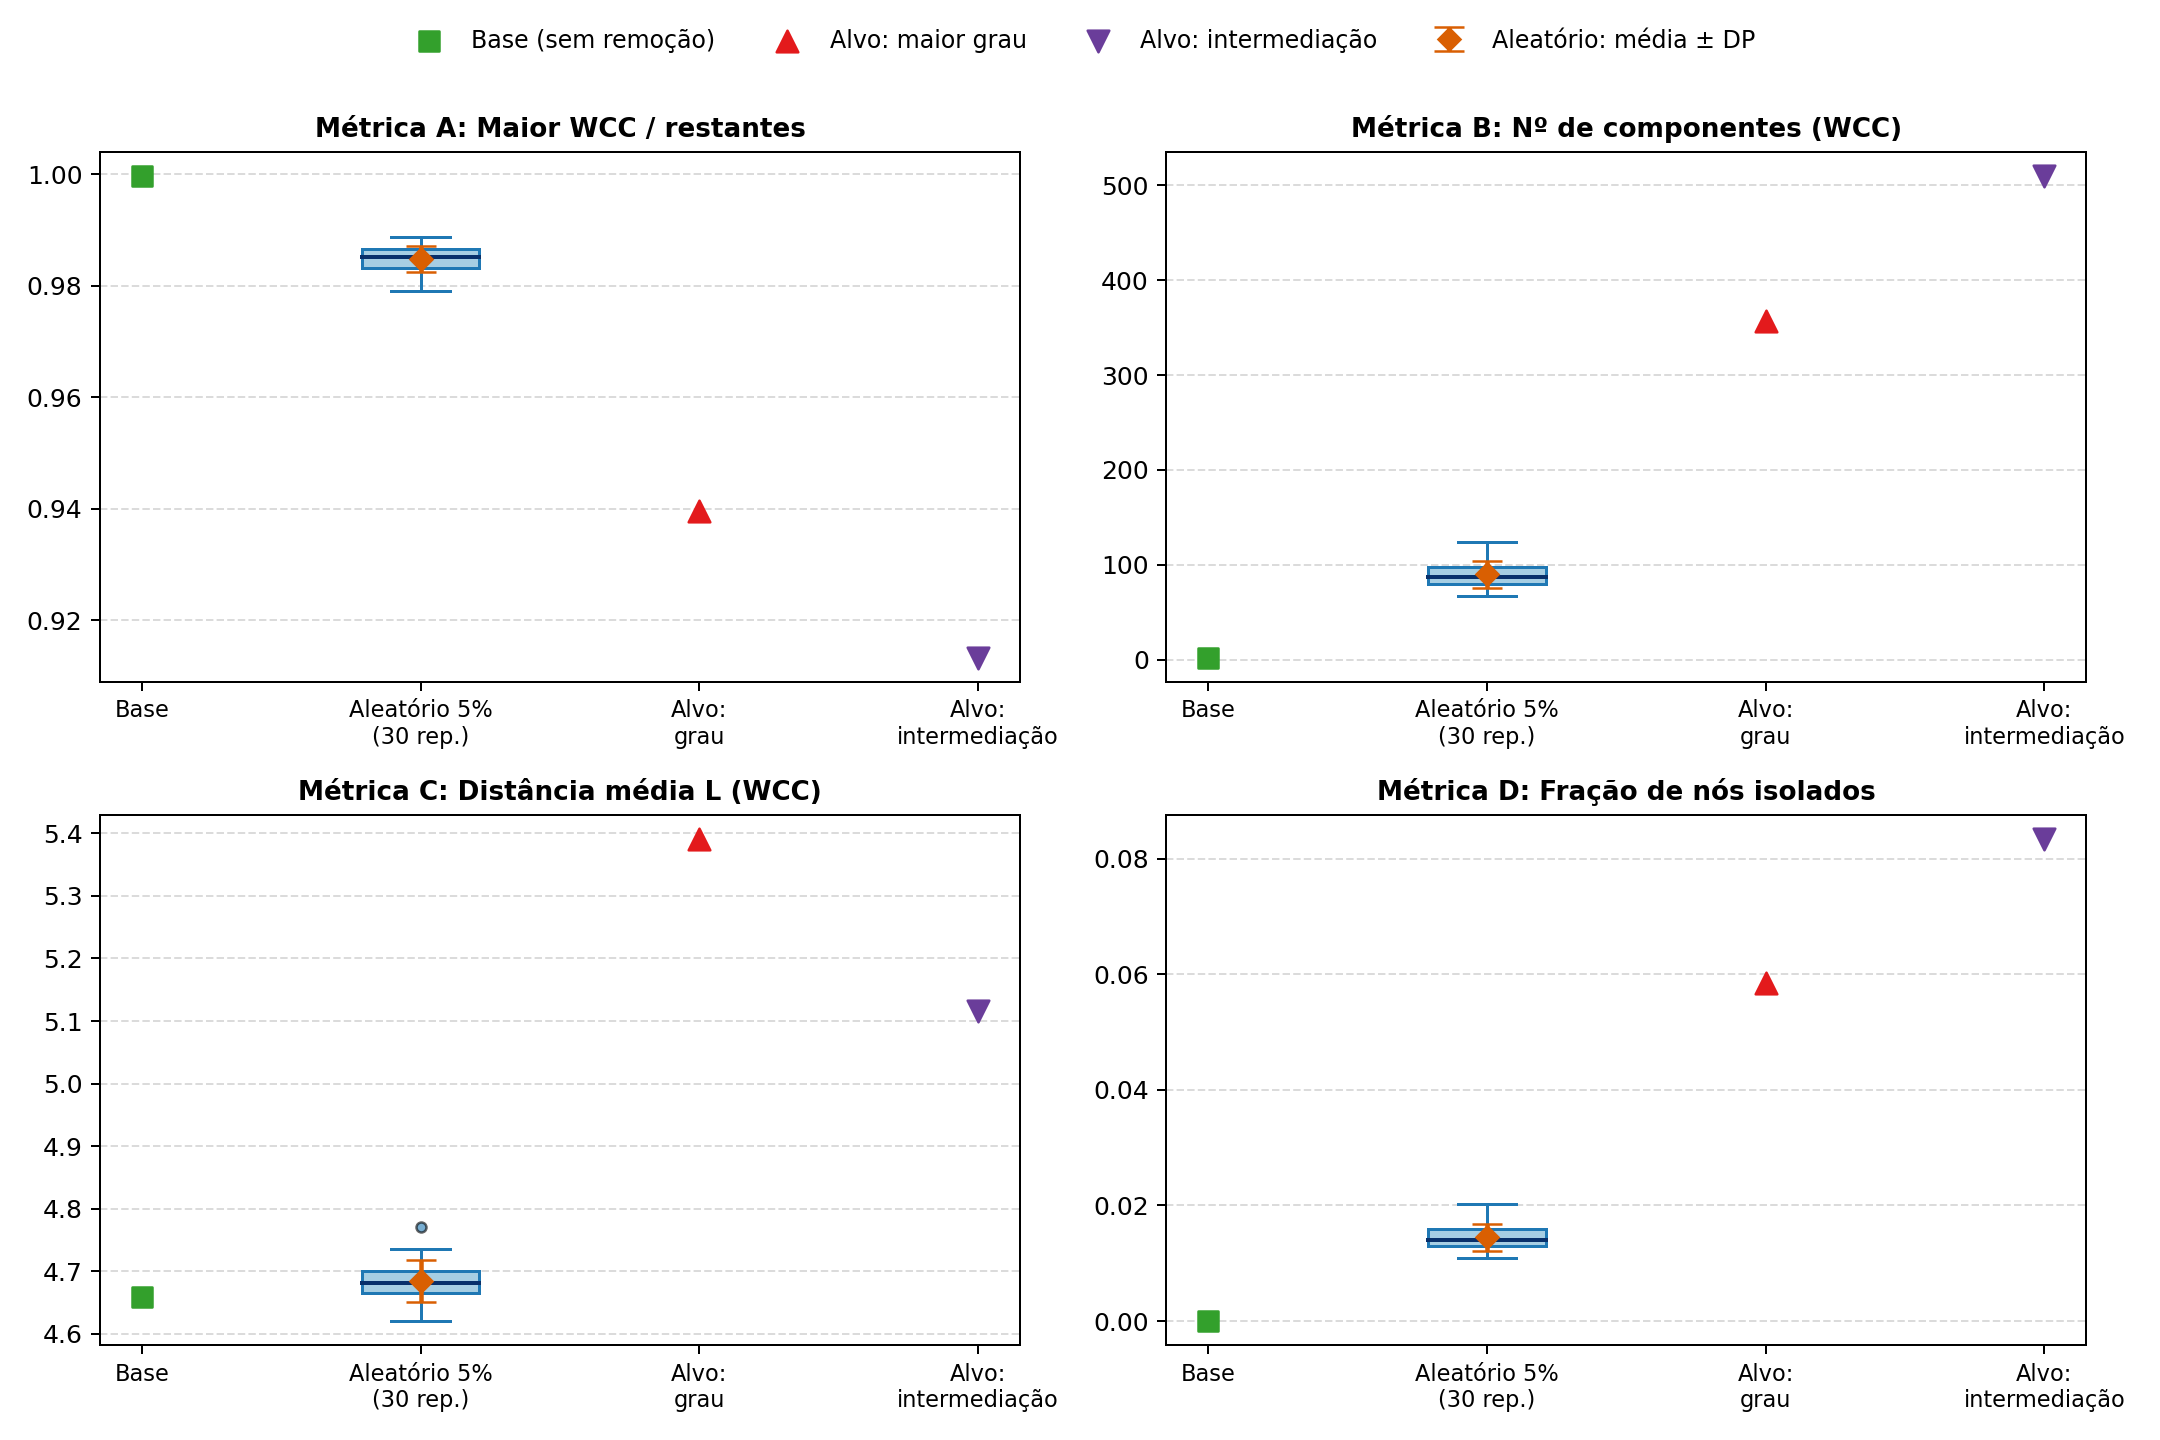
\includegraphics[width=0.92\textwidth]{robustez.png}
\caption{\emph{Boxplots} das 30 repetições de remoção aleatória de 5\% (com média $\pm$ desvio padrão em laranja) comparados ao grafo base e aos ataques direcionados por grau e por intermediação para as quatro métricas do Apêndice~C.}\label{fig:rob}
\end{figure*}
\noindent\textbf{(a) Remoção aleatória de 5\%: robusto.} Conforme a Tabela~\ref{tab:rob} e a Figura~\ref{fig:rob}, 98,5\% ($\pm 0{,}23$ p.p.) dos vértices restantes permanecem na maior componente fraca, $L$ sobe apenas de 4,66 para 4,68 ($\pm 0{,}03$, +0,5\%) e a eficiência cai 2\%. O número de componentes aumenta de 2 para 89,93 ($\pm 14{,}07$), quase inteiramente composto por nós isolados (86,8 $\pm$ 14,1 vértices, ou 1,45\% $\pm$ 0,23\% dos restantes). \textbf{(b) Remoção dos 5\% mais centrais: bem menos robusto.} Por grau ou por intermediação, a maior WCC cai para 94,0\% e 91,3\% dos restantes, o número de componentes salta para 357 e 510, e a fração de nós isolados atinge 5,85\% (350 vértices) e 8,34\% (499 vértices), respectivamente. Além disso, $L$ sobe 16\% e 10\%, e a maior SCC encolhe de 0,328 para 0,163 (por grau, queda de 50\%) e 0,193 (por intermediação, queda de 41\%). O \emph{ranking} por grau e por intermediação coincide em 163 dos 315 vértices. Mesmo assim, a rede não se desintegra: quase toda a fragmentação decorre do isolamento de nós periféricos de grau baixo, enquanto mais de 91\% dos vértices restantes permanecem conectados, o que é compatível com hubs de grau moderado (máximo 97) e sem um hub dominante.

\paragraph{4. Qual foi a descoberta mais interessante?}
O mais interessante foi a assimetria entre entrada e saída. \textbf{60,9\% dos \emph{peers} têm grau de saída 0, e entre os que têm saída positiva, 62\% têm exatamente 10 conexões de saída e 98,9\% têm no máximo 10.} Enquanto isso, o grau de entrada tem cauda pesada (máximo 91). Isso é o padrão que se esperaria de um limite de cerca de 10 conexões iniciadas por \emph{peer}, com os hubs sendo vértices que \emph{recebem} muitas conexões. Essa é uma hipótese consistente com os dados, não algo que os dados provem (não há metadados no arquivo). A consequência estrutural é concreta: o grafo dirigido tem 4.234 componentes fortes, das quais 4.233 são vértices isolados, e só 32,8\% dos vértices estão na maior SCC. Junto com o aviso do cabeçalho do arquivo (cada par é salvo uma vez), isso mostra que a orientação não deve ser tratada como relação simétrica nem como fluxo real de informação sem cautela.

\paragraph{5. (Extra) O grafo se aproxima de algum modelo clássico?}
\begin{table}[t]\centering\scriptsize
\caption{Comparação com modelos clássicos de mesmo $n$ e número de arestas semelhante (média de 5 réplicas).}\label{tab:mod}
\begin{tabular}{lrrrr}\toprule
Modelo & $C$ & $L$ & Grau máx. & DP grau \\\midrule
Grafo real & 0,0109 & 4,64 & 97 & 8,54 \\
Erdős--Rényi $G(n,m)$ & 0,0011 & 4,85 & 18 & 2,58 \\
Barabási--Albert ($m\approx3{,}3$) & 0,0087 & 3,99 & 269 & 9,19 \\
Watts--Strogatz ($k=6$, $p=0{,}1$) & 0,446 & 8,18 & 10 & 0,75 \\\bottomrule
\end{tabular}
\end{table}
\noindent \textbf{O mais próximo é Barabási--Albert, mas a aproximação é imperfeita.} O grafo real tem desvio de grau 8,5 e clustering 0,011, valores próximos aos do BA (9,2 e 0,009) e muito diferentes dos do ER (2,6 e 0,001) e do WS (0,75 e 0,45). Em contrapartida, o BA superestima o grau máximo (269 contra 97) e dá caminhos mais curtos (3,99 contra 4,64): os hubs reais são mais limitados, coerente com o patamar da CCDF e com a ideia de capacidade finita por \emph{peer}. O Watts--Strogatz está descartado (clustering 40 vezes maior e caminhos 76\% maiores). O Erdős--Rényi acerta o $L$ mas não a heterogeneidade dos graus.

\section{Discussão crítica}
\begin{itemize}
\item \textbf{Um único instantâneo.} O SNAP tem 9 instantâneos de agosto de 2002; este é só um. As conclusões valem para esse momento da rede.
\item \textbf{Semântica da orientação.} Como cada par é salvo uma vez, a orientação pode refletir a ordem de descoberta ou de conexão, não um fluxo. Medidas dirigidas (SCC, diâmetro 20, eulerianidade) devem ser lidas com essa ressalva; as não-dirigidas são mais seguras.
\item \textbf{Estimativas por amostragem.} As distâncias da Parte I são exatas (BFS de todos os vértices). Já $L$ nos modelos nulos usa 300 fontes por réplica e 5 réplicas, e a intermediação usa 500 fontes; os ataques são estáticos. Os resultados de robustez por intermediação são, portanto, aproximados.
\item \textbf{Lei de potência.} Não foi feito o teste de aderência por \emph{bootstrap}, a comparação com a log-normal ficou no limite do parâmetro e o grau de saída não segue o modelo. A conclusão ``cauda pesada, mas não lei de potência estrita'' é a que os dados sustentam.
\item \textbf{Medição de tempo.} Python tem variação entre execuções (o BFS/DFS/Dijkstra têm IC largo), os subgrafos de teste vêm de uma BFS a partir do hub e por isso são mais densos que o grafo médio (por exemplo, $n=500$ tem 3.460 arestas, 6,9 por vértice, contra 3,3 no total), e o Floyd-Warshall usa \texttt{numpy} para as atualizações internas. Os expoentes empíricos são, por isso, indicativos.
\item \textbf{Pesos.} Como o grafo é sem pesos, Dijkstra, Bellman-Ford e Floyd-Warshall com peso 1 não mostram a diferença que teriam com pesos reais, e os pesos aleatórios da MST são artificiais.
\end{itemize}

\section{Conclusão}
O p2p-Gnutella08 é uma rede esparsa (densidade $10^{-3}$), quase toda conectada (6.299 de 6.301 vértices na maior componente fraca) e de diâmetro pequeno (9; 99,95\% dos pares a até 7 saltos). Tem indício fraco de \emph{small-world} (clustering baixo em valor absoluto, mas maior que o aleatório), cauda de graus pesada, porém não uma lei de potência estrita, e é robusto a falhas aleatórias mas vulnerável a ataques direcionados aos hubs, que reduzem a maior componente forte em 41\% a 50\%. A característica mais marcante é a assimetria entre entrada e saída (60,9\% sem saída, e limite de cerca de 10 conexões de saída), que torna o grafo dirigido pouco fortemente conexo (32,8\%) e sugere cautela ao interpretar a orientação. Entre os modelos clássicos, o Barabási--Albert é o mais próximo. Na Parte II, os algoritmos lineares confirmaram $O(n+m)$, o Floyd-Warshall confirmou $O(n^3)$ e o Bellman-Ford ficou muito abaixo do pior caso por causa da parada antecipada.

\nocite{clauset2009,humphries2008}
\begin{thebibliography}{9}
\bibitem{leskovec2007} J. Leskovec, J. Kleinberg e C. Faloutsos. Graph Evolution: Densification and Shrinking Diameters. \emph{ACM TKDD}, 1(1), 2007.
\bibitem{ripeanu2002} M. Ripeanu, I. Foster e A. Iamnitchi. Mapping the Gnutella Network: Properties of Large-Scale Peer-to-Peer Systems and Implications for System Design. \emph{IEEE Internet Computing}, 2002.
\bibitem{clauset2009} A. Clauset, C. R. Shalizi e M. E. J. Newman. Power-law distributions in empirical data. \emph{SIAM Review}, 51(4), 2009.
\bibitem{humphries2008} M. D. Humphries e K. Gurney. Network ``small-world-ness'': a quantitative method for determining canonical network equivalence. \emph{PLoS ONE}, 3(4), 2008.
\end{thebibliography}
\end{document}
